%\documentclass{book}
\documentclass{report}


\usepackage{graphicx}
\usepackage{moreverb}
\usepackage{amsmath}
\usepackage{alltt}
\usepackage{rotating}
\usepackage{subfigure}
\usepackage{toc}
\usepackage{xspace}

\newcommand{\extref}[1]{$\S$\ref*{#1}}   % No hyperlink. For external refs. \extref
\newcommand{\comma}{\> ,}
\newcommand{\period}{\> .}
\newcommand{\wt}{\widetilde}
\newcommand{\grv}{\textasciigrave}
\newcommand{\hyperbf}[1]{\textbf{\hyperpage{#1}}}
\newcommand{\Ss}{\(^*\)}
\newcommand{\Dd}{\(^\dagger\)}

\newcommand{\AND}{&& \hskip -17pt\relax}
\newcommand{\CR}{\\}
\newcommand{\CRNO}{\nonumber \\}
\newcommand{\dstyle}{\displaystyle}

\newcommand{\Begineq}{\begin{equation}}
\newcommand{\Endeq}{\end{equation}}
\newcommand{\NoPrint}[1]{}

\newcommand{\pow}[1]{\cdot 10^{#1}}
\newcommand{\Bf}[1]{{\bf #1}}
\newcommand{\bfr}{\Bf r}

\newcommand{\bmad}{{\sl Bmad}\xspace}
\newcommand{\tao}{{\sl Tao}\xspace}
\newcommand{\mad}{{\sl MAD}\xspace}
\newcommand{\cesr}{{\sl CESR}\xspace}

\newcommand{\sref}[1]{\S\ref{#1}}
\newcommand{\Sref}[1]{Sec.~\sref{#1}}
\newcommand{\cref}[1]{Chapter~\ref{#1}}

\newcommand{\Newline}{\hfil \\ \relax}

\newcommand{\eq}[1]{{(\protect\ref{#1})}}
\newcommand{\Eq}[1]{{Eq.~(\protect\ref{#1})}}
\newcommand{\Eqs}[1]{{Eqs.~(\protect\ref{#1})}}

\newcommand{\vn}{\ttcmd}           % For variable names
\newcommand{\vni}{\ttcmdindx}
\newcommand{\cs}{\ttcmd}           % For code source
\newcommand{\cmd}{\ttcmd}          % For Unix commands
\newcommand{\rn}{\ttcmd}           % For Routine names
\newcommand{\tn}{\ttcmd}           % For Type (structure) names
\newcommand{\bn}[1]{{\bf #1}}       
\newcommand{\toffset}{\vskip 0.01in}
\newcommand{\rot}[1]{\begin{rotate}{-45}#1\end{rotate}}

\newcommand{\data}{{\mbox{data}}}
\newcommand{\reference}{{\mbox{ref}}}
\newcommand{\model}{{\mbox{model}}}
\newcommand{\base}{{\mbox{base}}}
\newcommand{\design}{{\mbox{design}}}
\newcommand{\meas}{{\mbox{meas}}}
\newcommand{\var}{{\mbox{var}}}

\newcommand\ttcmd{\begingroup\catcode`\_=11 \catcode`\%=11 \dottcmd}
\newcommand\dottcmd[1]{\texttt{#1}\endgroup}

\newcommand\ttcmdindx{\begingroup\catcode`\_=11 \catcode`\%=11 \dottcmdindx}
\newcommand\dottcmdindx[1]{\texttt{#1}\endgroup\index{#1}}

\newcommand{\St}{$^{st}$\xspace}
\newcommand{\Nd}{$^{nd}$\xspace}
\newcommand{\Th}{$^{th}$\xspace}
\newcommand{\B}{$\backslash$}
\newcommand{\W}{$^\wedge$}

\newcommand{\cbar}[1]{\overline C_{#1}}

\newlength{\dPar}
\setlength{\dPar}{1.5ex}

\newenvironment{example}
  {\vspace{-3.0ex} \begin{alltt}}
  {\end{alltt} \vspace{-2.5ex}}

\newcommand\Strut{\rule[-2ex]{0mm}{6ex}}

\newenvironment{Itemize}
  {\begin{list}{$\bullet$}
    {\addtolength{\topsep}{-1.5ex} 
     \addtolength{\itemsep}{-1ex}
    }
  }
  {\end{list} \vspace*{1ex}}

\newcommand{\Section}[1]{\section{#1}\indent\vspace{-3ex}}

\newcommand{\SECTION}[1]{\section*{#1}\indent\vspace{-3ex}}

% From pg 64 of The LaTex Companion.

\newenvironment{ventry}[1]
  {\begin{list}{}
    {\renewcommand{\makelabel}[1]{\textsf{##1}\hfil}
     \settowidth{\labelwidth}{\textsf{#1}}
     \addtolength{\itemsep}{-1.5ex}
     \addtolength{\topsep}{-1.0ex} 
     \setlength{\leftmargin}{5em}
    }
  }
  {\end{list}}


\setlength{\textwidth}{6.25in}
\setlength{\oddsidemargin}{0.25in}
\setlength{\evensidemargin}{0.00in}
\setlength{\textheight}{8.5in}
\setlength{\topmargin}{0in}

\begin{document}

%----------------------------------------------------------------
% Cover Page

\thispagestyle{empty}

\begin{flushright}
\large
  Revision: 0.1 \\
  9 June, 2004 \\
\end{flushright}

\vfill

{
\begin{center}
{\Huge \sf\bf The} \\
\vskip 0.1in
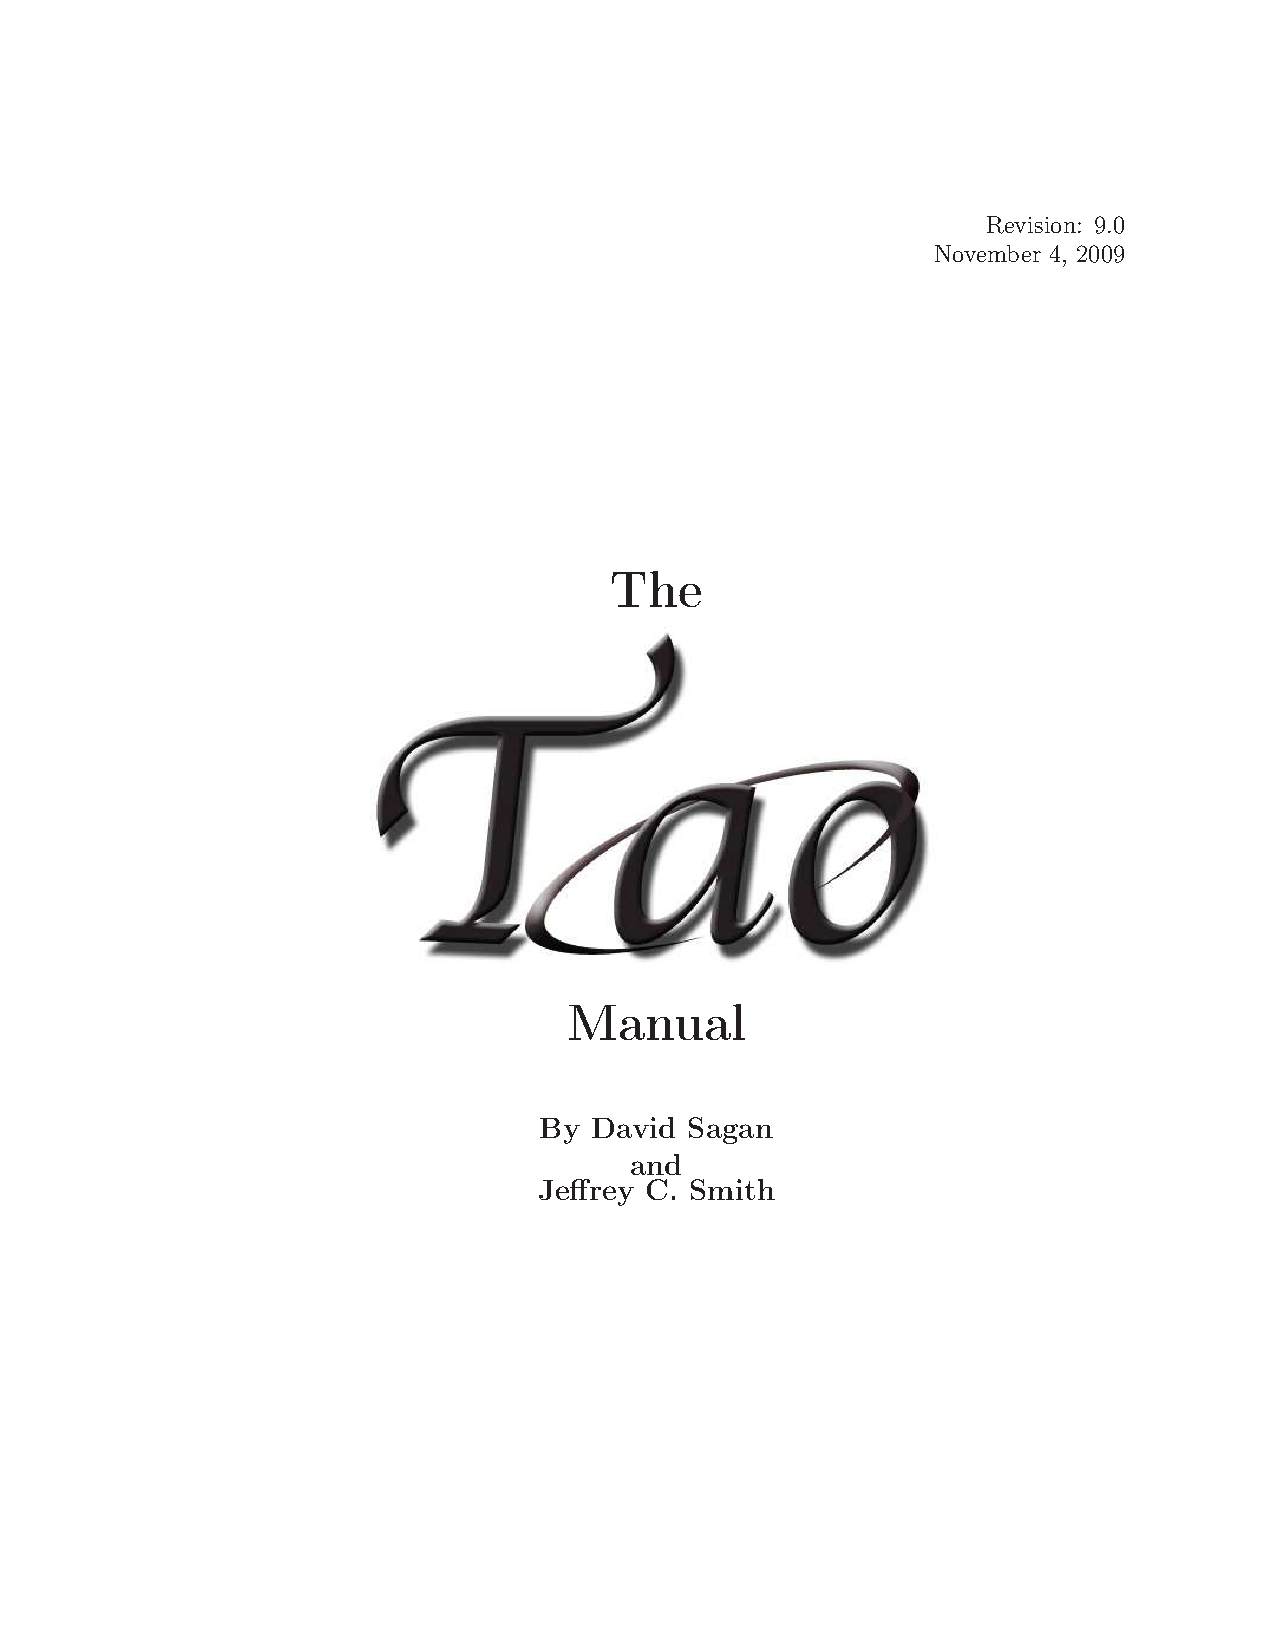
\includegraphics[width=10cm]{tao.psfig} \\
\vskip 0.1in
{\Huge \sf\bf Tutorial} \\
\vskip 0.1in
{\normalsize \sf\bf by Jeffrey C. Smith} \\
\end{center}
}

\vskip 1in
\begin{center}
{\Huge \bf *** VERY ROUGH DRAFT ***}
\end{center}
\vfill
\break
%----------------------------------------------------------------
%Introduction

{
\setlength{\parskip}{\dPar}
\setlength{\parindent}{0ex}

\section*{Tao: The Tool for Accelerator Optics}

The \tao program was developed
to reduce the time needed to develop working programs. \tao is a
machine independent program that implements the essential ingredients
needed to solve simulation problems. To make the
connection, \tao uses configuration input files that can be tailored to
specific machines. Additionally, \tao has been built
to be easily customizable so that extending \tao to solve new and
different problems is relatively straight forward.

More information can be found at the \bmad web site at
\begin{example}
  http://www.lepp.cornell.edu/~dcs/bmad
\end{example}

Tutorials are always difficult to write. Please send any recommendations 
for imporvement or notices of out-right errors to:
\begin{example}
  Jeff Smith <js344@cornell.edu>
\end{example}
}

%----------------------------------------------------------------
\tableofcontents
\listoffigures
%% \listoftables

\setlength{\parskip}{\dPar}
\setlength{\parindent}{0ex}

\part{``Vanilla'' \tao}
\label{p:vanilla_tao}

%----------------------------------------------------------------
\chapter{Before we start}
\label{c:before_beginning}

\tao is readily customizable. All the bookkeeping has already been done and all
you need to do custom analysis is write the subroutines perinent to your
project. However beginners are advised to start with
``out of the box'' \tao while getting to know the program. This tutorial will
guide you through the basic features of this ``vanilla'' \tao and then show you
how to customize \tao for your speciffic purposes.

\section{Getting and Compiling \tao}

\tao is available in the \cesr CVS area. To checkout a copy type `\cmd{cvs co
tao'} in the directory from where you want to run \tao. If you don't have \cesr
CVS write permission then type `\cmd{cesrcvs co tao}'. This will check out a copy
but will not allow you to check in changes to the code. If you aren't at Wilson
Laboratory then contact David Sagan \cmd{<dcs16@cornell.edu>} to obtain a copy. 

From the newly created \cs{./tao} directory type `\cmd{gmake}' to create the
libraries and then type `\cmd{gmake -f M.tao}' to create
the ``vanilla'' \tao program. Vanilla \tao is the basic \tao program without any
user customizations. If you are using a custom version of \tao then
follow the compiling directions from the custom \tao author. Keep in mind that
command syntax and usage may vary between custom versions of \tao (this is a
\textit{feature} \textbf{not} a bug!).

Once \tao has compiled go to the subdirectory \cs{./program} and type
\cmd{../../bin/tao} to run ``vanilla'' \tao. This directory contains all the
configuration files to get everything working. The first time you run the
program it will need to create a digested \bmad lattice file for the included
lattice. This may take a few minutes.

\subsection{Customising \tao}

After you are familiar with the basics of \tao you are ready to fully exploit
the versatility of this wonderful program. See part~\ref{p:custom_tao} to learn
how to do this.

%----------------------------------------------------------------
%----------------------------------------------------------------
\chapter{In the Beginning...}
\label{c:beginning}

%----------------------------------------------------------------
\section{There was the the user}

Part~\ref{p:vanilla_tao} assumes you are already familiar with basic particle beam
dynamics and its formalism. There are several books that introduce the topics
very well. The best the author has found so far is \textit{The Physics of
Particle Accelerators} by Klaus Wille. 

\tao is based on the \bmad subroutine library and you should have
a working knowledge of the conventions used by \bmad. \tao can be used ``out of
the box'' so an understanding of the nitty-gritty details of \bmad is not
necessary, however, one should be familiar with the material in Part I
of the \bmad manual.

First of all, what's \tao good for? Well, everything. It's versatility is that
it's easily exapandable. Think of it as an accelerator design and analysis
environment. the entire \bmad library is at your disposal.But even without any 
customizations \tao will do much analysis. These problems fall into three main
catagories:

\begin{itemize}
\item 
You want to design a lattice subject to various constraints.
\item 
You have some measured data and you want to make a correction. For
example, you want to know what steering strength changes will make an orbit
flat.
\item
You want to simulate what happens to the orbit, beta function,
etc., when you change something in the machine.
\end{itemize}

Programs that are written to solve these types of problems have common
elements: You have variables you want to vary in your model of your
machine, you have "data" that you want to view, and, in the first two
categories above, you want to match the machine model to the data (in
designing a lattice the constraints correspond to the data).

This tutorial is designed to get the user up and starting with \tao without
needing to dredge through the entire reference manual. Full command syntax
or greater detail on any topic can be found in the referencereferenc  manual.

%----------------------------------------------------------------
\section{Then there was the Super-universe}

Everything known to \tao is placed in an area called the
\textit{super-universe}. Within the \textit{super-universe} lies one or more
universes each containing a particular machine lattice. This allows for the user
to do analysis on multiple machines or multiple configurations of a single
machine at the same time. A \textit{super-universe} consists of the following
parts:

\subsection{A typical universe}
A universe contains a \bmad lattice plus whatever data one wishes to study
within this lattice (i.e. twiss parameters, orbit, phase \&etc...) . Actually,
there are three lattices within each universe: the \textbf{design
lattice}, \textbf{model lattice} and \textbf{base lattice}. \emph{All lattice changes
specified during a \tao session are incurred on the model lattice.} The design lattice is
fixed at initilization time and serves as a reference point for any elemental
changes incurred during the \tao session. The base lattice also serves as a
reference point but the user can transfer the model lattice over to the base
lattice at any time to create your reference lattice.

Each data point (for example, the horizontal orbit at some detector) has 5 datum
 quantities associated with it: the \textbf{measured data}, \textbf{reference
data}, \textbf{model data}, \textbf{design data} and \textbf{base data}. The
model, design and base data areas correspond to the appropriate quantity
calculated in their respective lattice above. The measured data corresponds to 
data obtained during a measurement. If doing design work then the desired data
value would be placed here. This data area is also refered to as the constraint during
optimization. The reference data is for looking at changes in the data with
respect to a reference.

\subsection{Variables}

Variables control attributes of elements in the model lattice of one or more
universes. So, a given variable may control a single attribute of one element
for one or more universes. These are what you vary in order to change
your model lattice. You can also change your model lattice by directly changing
and lattice element parameter. However, if you plan on doing any optimization then 
you will need to use the variables.

\subsection{Key Bindings}

Key bindings are used in \textit{single mode} where each key
stroke is interpreted without the user having to press the carriage control key.
Each group of keys is bound to a different variable and pressing these keys will
allow you to rapidly change your lattice optics.

\subsection{Other stuff in the Super-universe}

The super-universe also contains information pertaining to global environment variables and
plotting. No need to go into the details here. The \tao reference manual will
tell you all about this.

%----------------------------------------------------------------
%----------------------------------------------------------------
\chapter{Initializing \tao}
\label{c:initializing}

Initialization occurs at startup. There are \emph{four} files used to initialize \tao.
  \vspace*{-3ex}
\begin{description}
  \item[\textit{your lattice file}] \Newline
    This is your lattice file. ``Vanilla'' \tao comes with its own for
demonstration purposes.
  \item[tao.init] \Newline 
    This is where global environment variables, data/variable
arrays and key bindings are specified.
  \item[tao\_plot.init] \Newline
    This is where plotting is set up.
  \item[tao.startup (optional)] \Newline
    This is a command file that is read in after initialization. Any commands you
want entered in \tao everytime you start up are put here. This is also a great
place to define aliases.
\end{description}

There is no need to go into the details of the initialization files here. If
using vanilla \tao these are already set up for you in \cs{tao/program} and will
setup \tao for use with the included \cesr lattice. If
using a custom version of \tao then the customized \tao author will have already set something
up for you to use. If he or she didn't then go complain to him or her for making
your life difficult and demand proper treatment. If he or she still refuses to
do this for you then it looks like you'll need to read part~\ref{p:custom_tao}
of this tutorial!

\textbf{NOTE: the following chapters will work with vanilla \tao. The commands
entered and plotting output may be different for custom versions.}


%----------------------------------------------------------------
%----------------------------------------------------------------
\chapter{Getting information from \tao}
\label{c:get_info}

%----------------------------------------------------------------
\section{The plotting window}

When \tao first starts up you will see a plot window and a command prompt. 
Figure~\ref{f:plot_begin} shows what you will see in the plot window. In the top
two plots you see the \vn{x} and \vn{y} model lattice orbit data. The horizontal
axis is the \cesr BPM index. The horizontal pretzel and L03 vertical bump can be clearly 
seen. The slight vertical displacement due to the solenoid can also be seen around 
the IP. The orbit data is for the closed orbit electron (this being a storage
ring). The bottom two plots show the relative 
particle phase. That is, the difference
between the model and design phases (as documented in the plot title as [model -
design]. 

As a first step let's view the absolute model phase. At the \cmd{TAO>} prompt type
\begin{example}
  plot bottom model
\end{example}
This will change the data plotted in the bottom two graphs to just the model.
The plots are now way off scale. Let \tao automatically set the scale by typing
\begin{example}
  scale bottom
\end{example}
As expected, the phase increases approximately linearly as the particle travels
through the ring. Zero phase is halfway through the ring (at L03 in \cesr lingo).
This is always true. Absolute phase is arbitrary so \tao sets the average
phase to zero when generating the data. OK, lets' set this back to relative
phase by typing
\begin{example}
  plot bottom model - design
\end{example}


Let's now look at the beta function by typing
\begin{example}
  place bottom beta
\end{example}
Again, we need to rescale the plots by typing
\begin{example}
  scale bottom
\end{example}
We see the periodic FODO beta function where large horizontal beta corresponds to
small vertical beta and vice versa.

Likewise, we can look at the dispersion in the top two graphs by typing
\begin{example}
  place top eta
  scale top
\end{example}
The plot window should now look like Figure~\ref{f:plot_eta_beta}.

Now let's look at the coupling (C-matrix) by typing
\begin{example}
  place bottom coupling
  scale bottom
\end{example}
We see that there is strong coupling within the CLEO solenoid and virtually no
coupling anywhere else.

The x-axis is currently the BPM index number. It is sometimes convenient to plot
the data versus the longitudinal position. This is done by typing
\begin{figure}
  x-axis all s
\end{example}
The \cmd{all} will apply the change to all plot areas (both top and bottom). In
any of the above commands the \cmd{top} or \cmd{bottom} coulf have been replaced
with \cmd{all}.

\begin{figure}
  \centering
  \includegraphics[width=5in]{plot_page1.psfig}
  \caption{The plot window at startup}
  \label{f:plot_begin}
\end{figure}

\begin{figure}
  \centering
  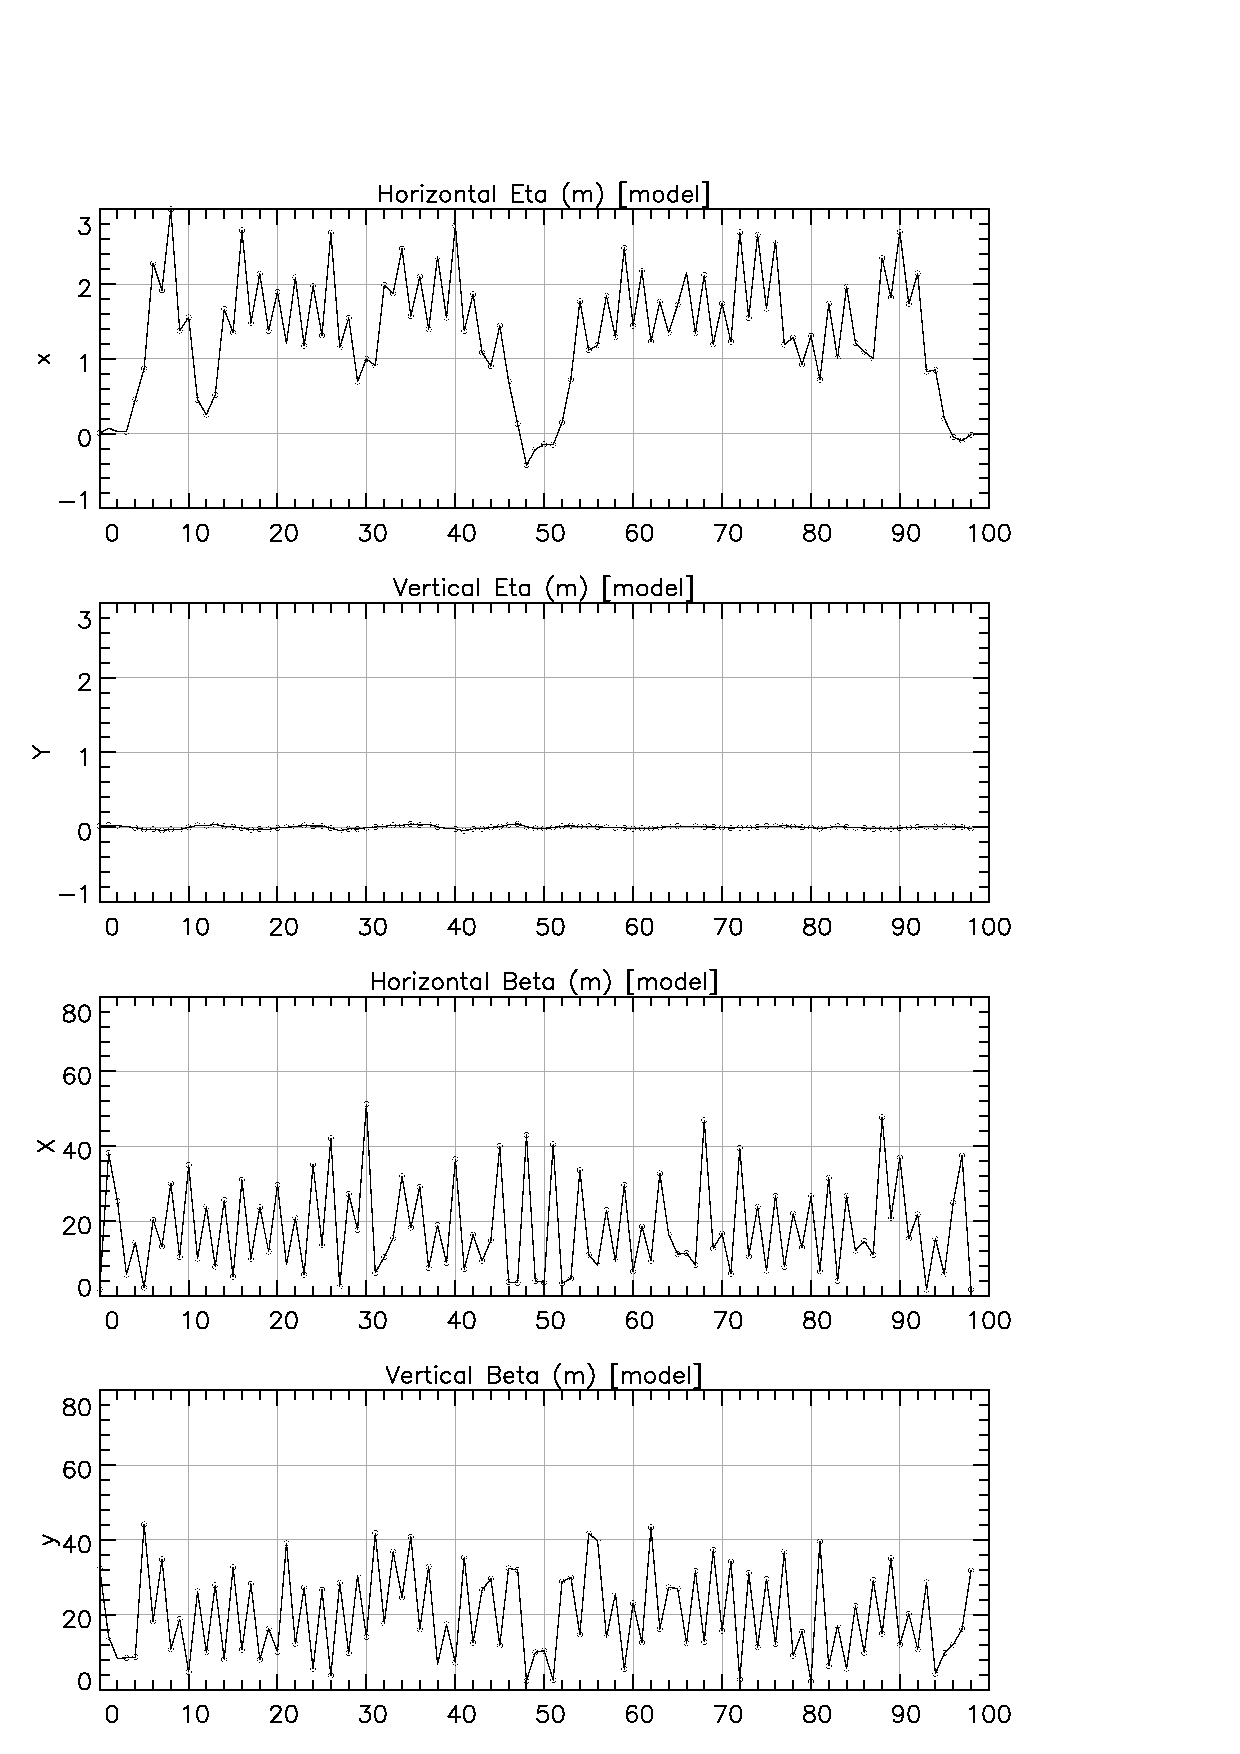
\includegraphics[width=5in]{plot_eta_beta.psfig}
  \caption{Plotting dispersion and beta function}
  \label{f:plot_eta_beta}
\end{figure}

%----------------------------------------------------------------
\section{the \cmd{show} command}

Anything in the super-universe can be displayed using the \cmd{show} command. To
get a list of the data elements currently defined in \tao type
\begin{example}
  show data
\end{example}
the output should look like:
\begin{example}
   1  orbit
   2  phase
   3  eta
   4  beta
   5  cbar
   6  coupling
\end{example}
There are 6 data types defined in the initialization file. The fifth and sixth are 
closely related. See the manual for an explanation.

To see the data values for the horizontal beta function for \cesr BPMs 1 through
50 type
\begin{example}
  show data beta:x 1:50
\end{example}
since we haven't changed any elements in the lattice yet the model values equal
the design values.

You can also view variables by typing
\begin{example}
  show var
\end{example}
To view the quadrupole k1 values for \cesr quadrupoles 5  and 20 through 30 type
\begin{example}
  sho var quad\_k1 5 20:30
\end{example}
Again, since we haven't changed any quadrupoles the model values are all at their
design values.

You can also see the details of a particular lattice element. To view the details
for quadrupole Q05W type
\begin{example}
  sho ele Q03W
\end{example}

A list of lattice elements between two elements can be shown by typing (for
example between elements BEGINNING and Q05W)
\begin{example}
  sho lattice beginning Q05W
\end{example}

Command line help is obtained by typing
\begin{example}
  help <command\_name>
\end{example}
where \<command\_name\> is the command you want help with.

%----------------------------------------------------------------
%----------------------------------------------------------------
\chapter{Modifying the lattice}
\label{c:modify_lattice}

Let's change a variable and see what happend to the lattice. We are going to
change a quadrupole strength so we should plot the change in beta and phase.
Type
\begin{example}
  place top beta
  plot top model - design
  place bottom phase
  scale
\end{example}

The k1 value can be increased by 0.01 units for quadrupole Q05W by typing
\begin{example}
  change var quad\_k1 5 0.01
  scale
\end{example}
Note the information returned after the command and the relative changes in
beta and phase in the plot window. This is a vertically focusing quadrupole so
the vertical beta and phase is affected more than the horizontal.

Let's put this quadrupole back where we found it. We can also modify the quadrupole
by modifying the element directly bytyping
\begin{example}
  change ele Q05W k1 -0.01
\end{example}

A great way to set all variable back to their design values is to type
\begin{example}
  set var all model = design
\end{example}

%----------------------------------------------------------------
%----------------------------------------------------------------
\chapter{Running the optimizer}
\label{c:optimizer}

There are two optimizers included with \tao. DESCRIBE THE OPTIMIZERS.

Let's mess the lattice up a little and see if the optimizer can ``fix'' the
lattice. First transfer the ``correct'' lattice to the \vn{meas} data area.
\begin{example}
  set data all meas = design
\end{example}
Now mess up the lattice a bit
\begin{example}
  change var quad\_k1 10 0.001
  change var quad\_k1 21 -0.001
  change var quad\_k1 67 -0.005
  plot all meas - model
  scale
\end{example}

Now specify what variable and data to use in the optimization. First type
\begin{example}
  show top10
\end{example}
to see what data is affecting the merit function the most. The merit function is
defined by
\Begineq
  {\cal M} \equiv \sum\_{i} w\_i \,
    \bigl[ \data\_\model(i) -  \data\_\meas(i) \bigr]^2 + 
  \sum\_{j} w\_j \,
    \bigl[ \var\_\model(j) - \var\_\meas(j) \bigr]^2
  \label{m1}
\Endeq
We see that the beta function is affecting the merit function the most. Since we
are looking at beta and phase let's only use that data in the optimization.
\begin{example}
  veto data all
  use  data beta all
  use  data phase all
\end{example}
We also know that we need to change quadrupoles to ``correct'' the lattice.
\begin{example}
  veto var all
  use var quad\_k1 all
\end{example}
Now let's see if we have the optimizer set up correctly.
\begin{example}
  sho optimizer
\end{example}
Whoops! we want to use the Levenberg-marquat optimizer so
\begin{example}
  set global optimizer = lm
  sho opt
\end{example}

Now we're ready to run or ``flatten'' the model to the data.
\begin{example}
  flatten
\end{example}
You see the optimizer going through its cycles and it did it! The model is now
``flattened.'' We can see what changes where done to the quadrupoles by typing
\begin{example}
  sho var quad\_k1
\end{example}
The optimizer didn't find the ``design'' lattice but changed more quadrupoles
than just 10, 21 anf 67. This isn't suprising. The optimizer finds the minimun
of the merit function and there are potentially many minimums. It does it's best
not to get stuck in a local minimum but as we can see by the plotted data, the
minimum found is very close to the design.

Alternatively, we could have used only a subsection of the quadrupole variables
by typing, for example,
\begin{example}
  use var quad\_k1 10 21 67
\end{example}
This will only use the the quadrupoles we modified. Now we see that the
optimizer put the quadrupole k1 values back to the design values.

%----------------------------------------------------------------
%----------------------------------------------------------------
\chapter{Single Mode}
\label{c:single_mode}

%----------------------------------------------------------------
%----------------------------------------------------------------
\chapter{Where to go from here}
\label{c:where_to_go}

%----------------------------------------------------------------
%----------------------------------------------------------------
%----------------------------------------------------------------
%----------------------------------------------------------------
\part{Customizing \tao}
\label{p:custom_tao}

%----------------------------------------------------------------
\end{document}
